\chapter{Modelo de Revisão de Percepções}

\noindent O modelo proposto para revisão de percepção é separado em três etapas, como mostra a figura \ref{fig:method}. Primeiro, o agente recebe um conjunto de percepções $p$ através de seus sensores. Depois disso, essas percepções passam através de uma função de refinamento, onde as percepções $p$ são refinadas tornando-se um subconjunto próprio $\rho$ de percepções refinadas. O conjunto $\rho$ é então passado para o módulo de alucinação e ilusão, onde cada percepção refinada passa por um processo de detecção de anomalia. As percepções de $\rho$ que forem consideradas válidas, irão constituir o subconjunto próprio $\varrho$ de percepções válidas, enquanto as anomalias formarão o subconjunto próprio $\sigma$ de anomalias. As percepções válidas são enviadas direto para o ciclo de raciocínio do agente, enquanto as anomalias irão cair em uma lista ordenada, onde aguardarão para passarem por um processo de planejamento automatizado.

Para ajudar a compreender o funcionamento desse modelo integrado ao raciocínio de um agente, nós usaremos uma versão estendida do exemplo \ref{example::robo}, um pouco mais complexa para podermos demonstrar passo a passo como funciona o modelo. 

\begin{example}
    Partindo do exemplo \ref{example::robo}, vamos supor que agora a loja vende estrelas lisas e listrados, que podem ser empacotadas com qualquer um dos pacotes. Além disso, o mesmo robô responsável por empacotar os itens que passavam por uma esteira é responsável por empacotar itens de três diferentes esteiras. As percepções são as mesmas que antes, mas agora ele é capaz de perceber os itens nas três esteiras, através de novos sensores táteis e de uma câmera que capta uma imagem aberta o suficiente para isso. As percepções continuam sendo do tipo \texttt{forma(textura)}.
    \label{example::robo2}
\end{example}{}

\begin{figure}[h!]
    \centering
    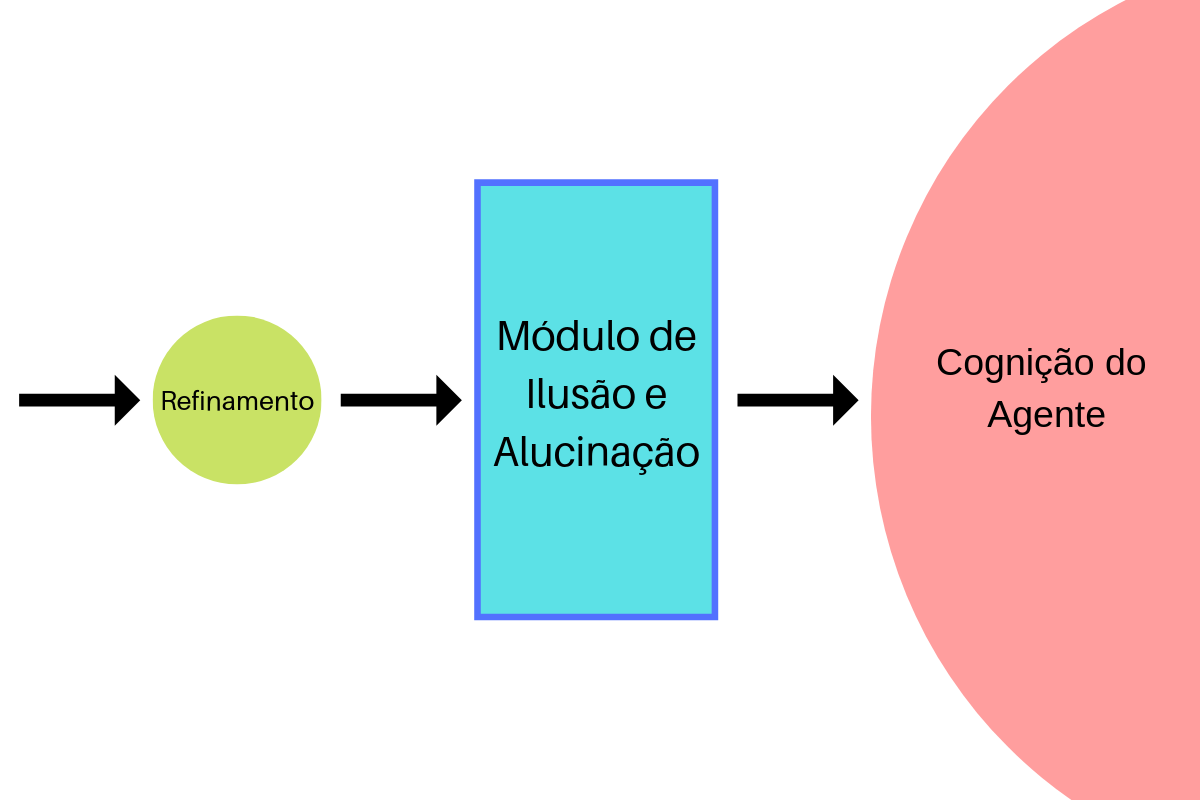
\includegraphics[width=0.8\textwidth]{Images/img2.png}
    \caption{Modelo de revisão de percepções.}
    \label{fig:method}
\end{figure}

\section{Módulo de refinamento}

O módulo de refinamento serve como uma primeira filtro para que percepções indesejadas pelo agente não cheguem até seu ciclo de raciocínio. O processo de refinamento é descrito pela definição \ref{def:refinamento}.

Caso não seja de interesse de uma determina arquitetura ou implementação de uma arquitetura refinar suas percepções, como pode ser o caso de um sistema especialista, o módulo de percepção pode simplesmente ter uma função tal que $f(x) = x$, com as percepções passando por dentro sem nenhum processo, possuindo assim o subconjunto próprio $\rho = p$.

\begin{example}
    Continuando o exemplo \ref{example::robo2}, as estrelas não fazem parte da área de atuação desse robô, e portanto para otimizarmos o processo de empacotamento é possível utilizar o módulo de percepções para refinar a informação recebida pelos sensores para enviar menos informações desnecessárias para a cognição do agente. Nesse exemplo, o robô pode ser implementado com uma função $\theta$ que realiza percepção ativa, removendo assim as percepções que não fazem sentido dentro do contexto em que ele está inserido. O conjunto de percepções $p$ passa pelo processo de percepção ativa e devolve $\rho$, que tem nesse caso específico, sendo $s$ o conjunto de percepções possíveis envolvendo estrelas, um comportamento tal que o conjunto $p$ sob a operação $\theta$ retorna $\rho = p \cap \overline{s}$. 
    Para tornar o processo mais tangível, vamos supor que o agente recebe o conjunto $p_i$ de percepções, composto por $\{circle(stripped), triangle(smooth), star(yellow)\}$. A operação $\theta$ vai remover de $p_i$ os elementos contidos no conjunto $s$ de possíveis percepções envolvendo estrelas, conforme foi descrito anteriormente. Portanto, a saída do bloco de percepções será $\rho = \{cicle(stripped), triangle(smooth)\}$.
    
\end{example}{}

\section{Módulo de Alucinação e Ilusão}

\begin{figure}[h]
    \centering
    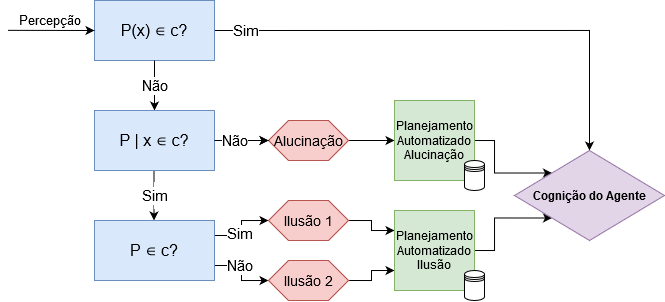
\includegraphics[width=0.8\textwidth]{Images/diagrama-modelo.png}
    \caption{Módulo de alucinação e ilusão.}
    \label{fig:model}
\end{figure}
 
 A figura \ref{fig:model} é a representação gráfica do módulo de alucinação e ilusão, que começa com a entrada $\rho$ sendo dirigida para o decisor 1. O primeiro decisor responde a pergunta: ``A percepção recebida está no código do agente?''. Caso a resposta for sim, consideramos a percepção como válida, e ela é enviada para a cognição do agente. Caso a resposta seja não, consideramos $\rho(x)$ uma anomalia, e enviamos ela para o segundo decisor, que responde a pergunta: ``O corpo ou o argumento do predicado $\rho(x)$ se encontra em alguma parte do código?''. Caso a resposta seja não, concluímos que a anomalia é uma alucinação. Caso contrário, ela é considerada uma ilusão e é enviada para o terceiro decisor. O terceiro decisor responde a pergunta: ``O corpo do predicado $\rho(x)$ está no código?''. Caso a resposta for sim, a ilusão é considerada uma ilusão classe 1, caso contrário, é considerado uma ilusão classe 2. Toda essa cadeia de decisores é representada pelo algoritmo abaixo:

\begin{algorithm}[H]
\SetKwInOut{Input}{input}
\Input{agent context \textit{c}, perception $\rho(x)$}

  \uIf{$\rho(x)$ is in \textit{c}}{
   $\rho(x)$ is a valid perception\;
   }\uElseIf{neither $\rho$ nor $x$ is in c}{
   $\rho(x)$ is a hallucination\;
   }\uElseIf{$\rho$ is in \texttt{c}}{
   $\rho(x)$ is an illusion class 1\;
  }\Else{$\rho(x)$ is an illusion class 2}
 \label{algorithm:decisor}
 \caption{Funcionamento dos decisores do módulo de ilusão e alucinação}
 \label{alg::selection}
\end{algorithm}

\begin{example}
    Para entender como as percepções são tratadas pelos decisores, vamos supor algumas entradas possíveis para o exemplo \ref{example::robo2}, que terão diferentes comportamentos ao longo do tempo de execução do nosso exemplo. Primeiro, vamos supor o caso mais básico, em que o agente recebe a percepção \texttt{quadrado(riscado)}. Essa é uma percepção completamente válida dentro do contexto do agente, pois ele possui um plano específico para tratar dessa percepção, que é empacotar o objeto com o papel vermelho. Portanto, nesse caso, $p(x) = \rho(x)$. Após sair do módulo de percepções, $\rho(x)$ passa como entrada para o decisor 1, que detecta que existe um plano específico para tratar da entrada, portanto a percepção é considerada válida e é diretamente enviada para a cognição do agente.

    Caso uma percepção não seja válida, ela é enviada para os decisores subsequentes, para que a anomalia seja devidamente classificada. 
\end{example}{}

\subsection{Bloco Avaliador}

Após a classificação da anomalia, ela é enviada para um bloco avaliador, que tratará de decidir qual anomalia pode ser considerada relevante para ocupar o planejamento automatizado e quais podem simplesmente retornar para o módulo de percepção para ajudar no processo de refinamento.
O funcionamento de um bloco avaliador deve permitir que alucinações ou ilusões seja processadas quando há tempo de processamento ocioso e o contexto permite. Para isso, vamos utilizar uma espécie de escalonador combinado com uma lista ponderada. Vamos considerar o tempo $c_m(\rho)$ o tempo médio de processamento gasto para cada percepção do conjunto $\rho$ recebido pelo agente, $a_m(\rho)$ o tempo médio do processamento das anomalias do conjunto $\rho$ recebida por um bloco de planejamento automatizado e $l_a$ a lista ponderada de $a$, onde $a$ é o índice que representa um dos três blocos avaliadores (de alucinação, ilusão classe 1 ou ilusão classe 2) utilizado para manter a generalidade. O principio do funcionamento da fila ponderada é o mesmo de uma fila comum, First in First Out (FIFO). Quando um elemento é inserido pela primeira vez na fila, ele recebe o peso 1. Quando uma cópia do mesmo elemento é inserida novamente, o elemento tem seu peso adicionado em 1, como mostra a figura \ref{filaPonderada}. Além disso, sendo $\rho$ o conjunto de percepções recebido pelo bloco de alucinação e ilusão, $|\rho|$ o número de percepções do conjunto e $\rho_a$ o número de anomalias.

O bloco avaliador seleciona quando uma percepção deve ser tratada através de uma função matemática, levando em conta o tempo médio de processamento de uma percepção válida e de uma anomalia, através da função de processamento. Além desse funcionamento básico, o bloco avaliador ainda contém um mecanismo para remover anomalias classificadas com irrelevantes para o sistema, através de uma função de limpeza. Caso essa função retorne verdadeiro, todos os elementos de peso 1 da sua respectiva lista são removidos. Essas duas funções serão trabalhadas na seção de formalismo.

\begin{figure}[h!]
    \centering
    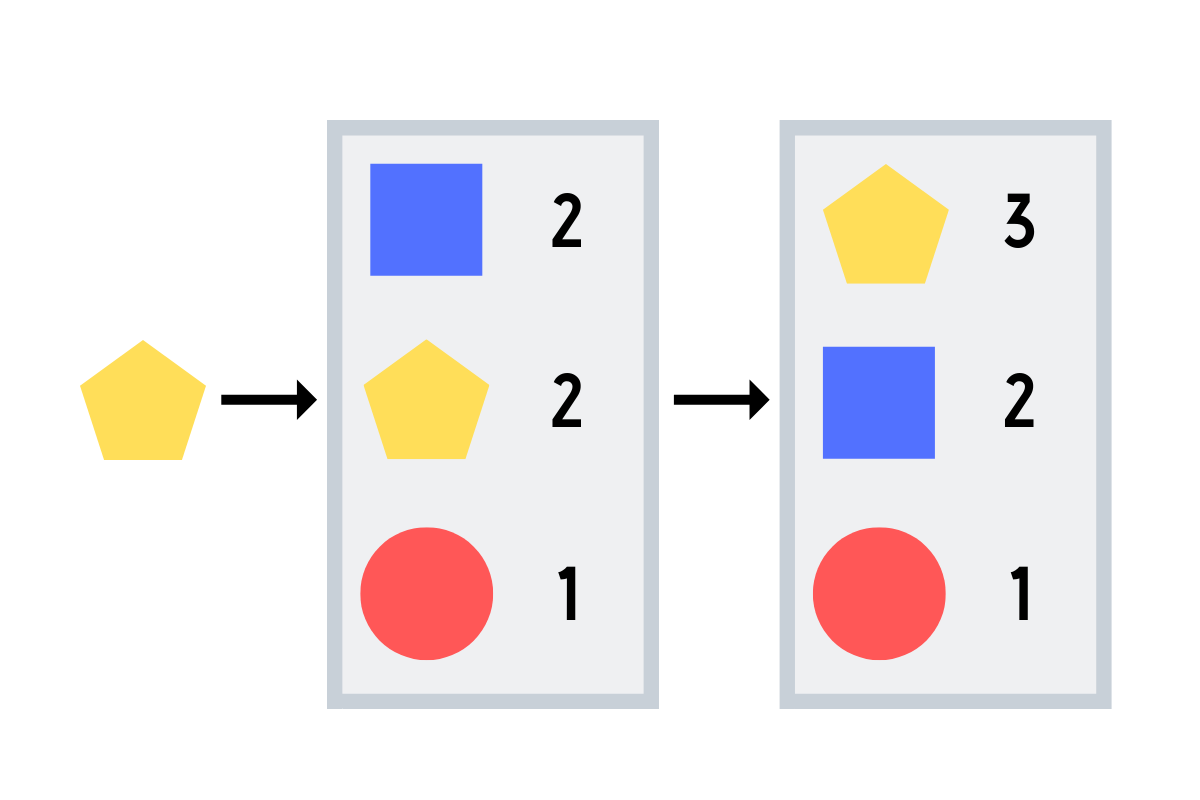
\includegraphics[width=0.49\textwidth]{Images/filaPonderada.png}
    \caption{Exemplo de fila ponderada.}
    \label{filaPonderada}
\end{figure}

\begin{example}
    Vamos supor que a percepção recebida pelo agente foi \texttt{lua(serrilhada)}. Lua não é um item que deveria ser percebido pelo agente, mas ou a implementação da percepção ativa foi simplória demais, simplesmente filtrando as estrelas, ou houve alguma falha que permitiu que ela chegasse ao módulo de alucinação e ilusão. Uma das propostas do modelo é detectar esse tipo de anomalia, que é uma falha completa do sistema. Quando ela chega ao decisor 1, é classificada como anomalia, pois não faz parte do escopo do agente. Em seguida, a percepção é enviada para o decisor 2, que verifica que não existe nenhuma menção de nenhuma parte da percepção no comportamento do robô, ou seja, é uma alucinação. Uma vez detectada a alucinação, a percepção segue para o bloco avaliador, onde será inserida na fila ponderada com o peso 1. Como consideramos apenas uma percepção recebida, e essa percepção é considerada uma anomalia, a equação da função de processamento é validada, e a anomalia segue para o bloco de planejamento automatizado.
\end{example}{}

\subsection{Bloco de Planejamento Automatizado}

O bloco de planejamento automatizado é potencialmente a parte mais custosa computacionalmente, e a parte mais difícil de ser implementada por todo o sistema. Um planejamento automatizado puramente simbólico tende a ser extremamente pesado, uma vez que pode considerar milhares de alternativas para o estado de mundo atual, tentando chegar mais perto de seu objetivo. Um processo de planejamento automatizado conexionista é uma opção, já que estamos tratando de uma análise incompleta do mundo, tratando do desconhecido. Teorias mais rebuscadas como criatividade computacional\cite{colton2012computational} podem ser adicionadas aqui, criando mais uma camada de complexidade para o agente, mas em troca dando um resultado ainda mais preciso para a avaliação da qualidade da percepção.

Uma percepção pode chegar ao bloco de planejamento automatizado quando ela for a primeira na fila ponderada e a função de processamento retornar verdadeiro. De um ciclo para outro, as percepções permanecem na fila, a não ser que sejam descartadas pelo mecanismo de limpeza. Nosso modelo não explicita qual é a ordem que os blocos avaliadores devem processar suas filas para mandar anomalias para o planejamento automatizado, ficando a cargo da implementação em questão tomar essa decisão.


\begin{example}
    Para mostrar o caminho que faz uma ilusão, vamos considerar que o agente recebe em duas esteiras a percepção \texttt{triangulo(listrado)}. Não existem triângulos listrados na loja, mas como $\theta$ não filtra essa percepção, ela vai chegar ao decisor 1. Como não existe um plano específico para tratar essa percepção, ela é considerada uma anomalia, e é encaminhada ao decisor 2. Como existe um plano para tratar de triângulos lisos, a percepção é então classificada como uma ilusão, e vai para o terceiro decisor. Nele, como o plano trata triângulos, a percepção é considerada uma ilusão classe 1. Finalmente após a percepção ter sido classificada corretamente, ela é enviada para o bloco avaliador, e é inserida na fila ponderada com peso 1. Depois disso, a percepção da segunda esteira, que é igual a que já foi tratada, chega ao bloco de alucinação e ilusão. Essa percepção vai fazer o mesmo caminho até o bloco avaliador e o peso da anomalia já presente na fila é aumentada para 2. Como duas percepções foram consideradas anomalias, vamos considerar que a função de processamento seja satisfeita, e o bloco avaliador passa essa anomalia para o bloco de planejamento automatizado.
    
    Após uma percepção ser considerada relevante para ser enviada ao planejamento automatizado, ela deve gerar um novo plano para aquela percepção a ser adicionada ao conjunto de planos do agente, e essa percepção então deixará de ser uma anomalia. Ilusões e alucinações tem blocos de planejamento automatizado separados para permitir que duas implementações completamente diferentes sejam utilizadas de acordo com a função do agente e a necessidade de criar novos planos eficientes. Retomando o exemplo dois, quando o planejamento automatizado de alucinações recebe a percepção \texttt{lua(serrilhada)}, um processo de planejamento automatizado deve ser executado. Para esse exemplo, consideremos um planejamento automatizado puramente simbólico, que analisa uma grande quantidade de estados futuros possíveis para o ambiente em que o robô está inserido e seleciona aquele que será mais eficiente para que o agente se aproxime de seu objetivo principal (terminar de empacotar os itens). Isso é extremamente custoso, mas como alucinações são muito raras para esse agente em questão, pois ele já tenta eliminar ao máximo percepções fora de seu escopo através da percepção ativa. Portanto, é um custo que vale a pena pois vai gerar um plano eficiente, evitando novas alucinações. No exemplo, é possível que a lua seja resultado de um corte errado na peça circular. Portanto, o agente precisa descartar esse item, para evitar gasto com embalagem desnecessária e que o item seja repassada para uma próxima etapa, gerando ainda mais custo. Assim, um novo plano da forma \texttt{lua(serrilhada) -> descartar} é adicionado, e \texttt{lua(serrilhada)} deixa de ser uma alucinação.

    No caso da percepção \texttt{triângulo(listrado)} do segundo exemplo, o agente poderia ter um bloco de planejamento automatizado baseado em uma rede baysiana, uma vez que ilusões podem ser muito mais comuns e o agente já tem uma breve noção do que deve ser feita com objetos do tipo. \texttt{triângulo(listrado)} pode ser um novo item a venda na loja, e como já foi verificado em duas esteiras diferentes, faz sentido que ele não seja uma mera falha de sensores. Assim, o planejamento automatizado pode inferir o plano \texttt{triângulo(listrado) -> empacotar}, permitindo que o agente tenha um aprendizado dinâmico resultado da adição de um novo plano em seu conjunto de planos. Assim como no caso da ilusão, uma vez que esse plano novo foi adicionado a percepção original deixa de ser uma anomalia, uma vez que faz parte do contexto em que o agente está trabalhando.

\end{example}{}
